%%%%%%%%%%%%%%%%%%%%%%%%%%%%%%%%%%%%%%%%%%%%%%%%%%%%%%%%%%%%%%%%%%%%%%%%%%%%%%%%%%%%%%%
\cleardoublepage
\thispagestyle{empty}
\begin{center}
\vspace*{3cm}
{\huge \bf Part I}\\ \vspace*{1cm}
{\Huge \bf Theoretic Foundations}\\\vspace*{0.2cm}
\begin{figure}[ht]
\centering
\includegraphics[height=6cm]{figures/part1_notesAndWaveform_orange}
\end{figure}
\end{center}
\addcontentsline{toc}{part}{I\hspace {1em}Theoretic Foundations}
\label{par:part1}
\newpage
\quad
\thispagestyle{empty}
\newpage

%%%%%%%%%%%%%%%%%%%%%%%%%%%%%%%%%%%%%%%%%%%%%%%%%%%%%%%%%%%%%%%%%%%%%%%%%%%%%%%%%%%%%%%


%%%%%%%%%%%%%%%%%%%%%%%%%%%%%%%%%%%%%%%%%%%%%%%%%%%%%%%%%%%%%%%%%%%%%%%%%%%%%%%%%%%%%%%
\chapter{Ordinary Differential Equations and Deep Learning}
\label{chapter:Foundations}
%%%%%%%%%%%%%%%%%%%%%%%%%%%%%%%%%%%%%%%%%%%%%%%%%%%%%%%%%%%%%%%%%%%%%%%%%%%%%%%%%%%%%%%

The aim of this work is to model analog audio effects using an \ac{ODE}-inspired approach to deep learning. This part of the thesis presents the theoretical background concerning these fields in the scope relevant for this work. 

In this chapter, in \Section{section:ode}, the \acp{ODE} are presented with a brief description of numerical methods used to solve them. In \Section{section:deep_learning}, the tools and methods from deep learning relevant for this thesis are presented. Finally, in the next chapter, the general concept of \ac{VA} modeling is presented.

%%%%%%%%%%%%%%%%%%%%%%%%%%%%%%%%%%%%%%%%%%%%%%%%%%%%%%%%%%%%%%%%%%%%%%%%%%%%%%%%%%%%%%%
\section{Ordinary Differential Equations}
\label{section:ode}
%%%%%%%%%%%%%%%%%%%%%%%%%%%%%%%%%%%%%%%%%%%%%%%%%%%%%%%%%%%%%%%%%%%%%%%%%%%%%%%%%%%%%%%

An \acf{ODE} is an equation of the form
\begin{equation}
  \frac{\mathrm{d} y}{\mathrm{d} t} = f(t, y),
  \label{eq:general_ode}
\end{equation}
where $y$ is the \emph{unknown function}, $t$ is the \emph{independent variable}, and $f(t, y)$ is a function of both, $t$ and $y$. Implicitly, $y$ is dependent on $t$, i.e., $y = y(t)$. In the scope of this work, $t$ denotes time. The term \emph{ordinary} means that $y$ is a function of a single variable and, thus, an "ordinary" derivative is used, i.e., $\frac{\mathrm{d} y}{\mathrm{d} t}$ \cite{Gockenbach2011}.

To \emph{solve} an \ac{ODE} means to find a function $y$ that satisfies \Equation{eq:general_ode}. Such $y$ is called a \emph{solution}.

\acp{ODE} are used to model dynamical systems \cite{Scheinerman1996,Karlsson2019}. A class of dynamical systems that can be described by an \ac{ODE} are electrical circuits containing capacitive elements. An example of such a system is the diode clipper circuit \cite{Yeh2007} discussed in \Chapter{chap:diode_clipper}.
Since an equation of the form \eqref{eq:general_ode} describes a rate of change $\frac{\mathrm{d} y}{\mathrm{d} t}$, its solution will not be a single function but rather a family of functions or a parametrized function. To obtain a unique solution, we need to specify an \emph{\ac{IC}}, i.e., the value of $y$ at some fixed point (typically at $t=0$). An \ac{ODE} together with an \acl{IC} makes up an \emph{\ac{IVP}}.

Some classes of \acp{IVP} can be solved analytically. However, for the most interesting applications, e.g., in the domain of analog audio effects, the corresponding \acp{IVP} are solved using numerical methods: algorithms using discrete points to approximate the true solution \cite{Gockenbach2011}. 

A group of numerical methods is called \emph{time-stepping methods}. Given a grid of time instants $t_0 < t_1 < \dots < t_n$ and a value of $y$ at $t_0$, $y(t_0)$, these methods use the following identity
\begin{equation}
  y(t_{i+1}) = y(t_{i}) + \int \limits_{t_i}^{t_{i+1}} f(\tau, y(\tau)) \mathrm{d} \tau
  \label{eq:time_stepping_identity}
\end{equation}
to approximate the value of $y$ at the points on the grid, $y(t_1), y(t_2), \dots, y(t_n)$. The core idea is to approximate the integral in \Equation{eq:time_stepping_identity}. Thus, the process of solving an \ac{IVP} is often referred to as \emph{integrating} the \ac{ODE} \cite{Gockenbach2011}.

What follows is a description of some of the numerical schemes used to approximate the integral in \Equation{eq:time_stepping_identity}.

%%%%%%%%%%%%%%%%%%%%%%%%%%%%%%%%%%%%%%%%%%%%%%%%%%%%%%%%%%%%%%%%%%%%%%%%%%%%%%%%%%%%%%%
\subsection{Forward Euler}
\label{subsection:forward_euler}
%%%%%%%%%%%%%%%%%%%%%%%%%%%%%%%%%%%%%%%%%%%%%%%%%%%%%%%%%%%%%%%%%%%%%%%%%%%%%%%%%%%%%%%

The simplest approximation of the integral in \Equation{eq:time_stepping_identity} is based on the \emph{left-endpoint rule} \cite{Gockenbach2011}

\begin{equation}
  \int \limits_{t_i}^{t_{i+1}} f(\tau, y(\tau)) \mathrm{d} \tau \approx f(t_i, y(t_i))\Delta t,
  \label{eq:forward_euler}
\end{equation}

where $\Delta t = t_{i+1} - t_i$.

It is important to note, that unless $y(t_i)$ is the initial value, it must be computed from previous time points. This results in error accumulation across time steps. The total error is on the order of the time step size $\Delta t$, which leads to the conclusion that in order to get a more accurate approximation with the forward Euler method, one needs to decrease the time step used \cite{Gockenbach2011}. In turn, decreasing the time step increases the number of computations needed to obtain the values of $y$ at the specified points.

The benefits of the Euler method are a straightforward implementation and the least amount of computations in comparison to other schemes.

Since we compute the solution according to the time steps ordering (\emph{forward} in time), this method is called an \emph{explicit} method.

%%%%%%%%%%%%%%%%%%%%%%%%%%%%%%%%%%%%%%%%%%%%%%%%%%%%%%%%%%%%%%%%%%%%%%%%%%%%%%%%%%%%%%%
\subsection{Explicit Runge-Kutta Methods}
\label{subsection:runge_kutta_methods}
%%%%%%%%%%%%%%%%%%%%%%%%%%%%%%%%%%%%%%%%%%%%%%%%%%%%%%%%%%%%%%%%%%%%%%%%%%%%%%%%%%%%%%%

The \ac{RK} methods are based on evaluating the function and the derivative in between the time steps. Thus, the approximation of the integral in \Equation{eq:time_stepping_identity} takes on the form \cite{Gockenbach2011}

\begin{align}
  \int \limits_{t_i}^{t_{i+1}} f(\tau, y(\tau)) \mathrm{d} \tau &\approx \Delta t \sum \limits_{j=1}^{m} \alpha_j k_j,\label{eq:rk_first}\\
  k_1 &= f(t_i, y(t_i)),\\
  k_2 &= f(t_i + \gamma_2 \Delta t, y(t_i) + \beta_{21} \Delta t k_1), \\
  k_3 &= f(t_i + \gamma_3 \Delta t, y(t_i) + \beta_{31} \Delta t k_1 + \beta_{32} \Delta t k_2),\\
  \vdots & \\
  k_m &= f(t_i + \gamma_m \Delta t, y(t_i) + \sum \limits_{l=1}^{m-1} \beta_{ml} \Delta t k_l), \label{eq:rk_last}
\end{align}
where
\begin{equation}
    \sum \limits_{j=1}^{m} \alpha_j = 1.
\end{equation}

$k_j$ are estimates of the derivative $f$ at $m$ nodes in the interval $[t_i, t_{i+1}]$, $\alpha_j$ are weights with which to sum the partial residuals $\Delta t k_j$. $\beta_\text{\underline{\hspace{2mm}}}$ coefficients have the same role for intermediate computations of $f$. $\gamma_j$ coefficients control which derivative approximations to use at specific nodes. For example, one could set $\gamma_j = \sum \limits_{l=1}^{j-1} \beta_{jl}$.

By fixing the values of the coefficients $\alpha_j, \beta_\text{\underline{\hspace{2mm}}}$, and $\gamma_j$, one obtains different numerical schemes. Their \emph{order} is the number of nodes used in between the steps. The most popular schemes are forward Euler (order 1), midpoint (order 2), \ac{RK}4 (order 4), and \ac{DOPRI} (using 4th and 5th order estimates). The values of the coefficients for the \ac{RK} methods are stored in \emph{Butcher tableaus} \cite{Atkinson2009}. The structure of a tableau corresponding to \EquationRange{eq:rk_first}{eq:rk_last}is shown in \Table{tab:rk_tableau}. A tableau for \ac{RK}4 is given in \Table{tab:rk4_tableau}.

\begin{table}
  \centering
  \caption{Generic \acl{RK} tableau.}
  \begin{tabular}{c | c c c c c}
    0 & & & & &\\
    $\gamma_2$ & $\beta_{21}$ & & & &\\
    $\gamma_3$ & $\beta_{31}$ & $\beta_{32}$ & & &\\
    $\vdots$ & $\vdots$ & & $\ddots$ & &\\ 
    $\gamma_m$ & $\beta_{m,1}$ & $\beta_{m,2}$ & $\dots$ & $\beta_{m,m-1}$ &\\ \hline
           & $\alpha_1$ & $\alpha_2$ & $\dots$ & $\alpha_{m-1}$ & $\alpha_m$ \\
  \end{tabular}
  \label{tab:rk_tableau}
\end{table}

\begin{table}
  \centering
  \caption{\ac{RK}4 scheme tableau.}
  \bgroup
  \def\arraystretch{1.5}%  1 is the default, change whatever you need
  \begin{tabular}{c | c c c c}
    0 & & & &\\
    $\frac{1}{2}$ & $\frac{1}{2}$ & & &\\
    $\frac{1}{2}$ & 0 & $\frac{1}{2}$ & &\\
    1 & 0 & 0 & 1 &\\ \hline
      & $\frac{1}{6}$ & $\frac{1}{3}$ & $\frac{1}{3}$ & $\frac{1}{6}$ \\    
  \end{tabular}
  \egroup
  \label{tab:rk4_tableau}
\end{table}

The accuracy of numerical solvers can be further improved by using an \emph{adaptive stepsize} (changing the size of the step according to the error estimate) or using \emph{multiple steps} (using more than one of the already computed values of $y$). Different modifications lead to different accuracy-performance trade-offs.

%%%%%%%%%%%%%%%%%%%%%%%%%%%%%%%%%%%%%%%%%%%%%%%%%%%%%%%%%%%%%%%%%%%%%%%%%%%%%%%%%%%%%%%
\subsection{Stiffness}
\label{subsection:stiffness}
%%%%%%%%%%%%%%%%%%%%%%%%%%%%%%%%%%%%%%%%%%%%%%%%%%%%%%%%%%%%%%%%%%%%%%%%%%%%%%%%%%%%%%%

An \ac{ODE} is said to be \emph{stiff} if it requires the explicit methods to use a very small time step in order not to become numerically unstable. Instead of sufficiently decreasing the time step, one may turn to \emph{implicit} methods which use future time steps to compute the previous ones.

A simple example of an implicit method is the \emph{backward Euler} method, which uses the \emph{right-endpoint rule} to approximate the integral in \Equation{eq:time_stepping_identity} \cite{Gockenbach2011}

\begin{equation}
    \int \limits_{t_i}^{t_{i+1}} f(\tau, y(\tau)) \mathrm{d} \tau \approx f(t_{i+1}, y(t_{i+1}))\Delta t.
  \label{eq:backward_euler}
\end{equation}

Using \Equation{eq:backward_euler} in \Equation{eq:time_stepping_identity} sometimes requires iterating between the two, while the first estimate of $y(t_{i+1})$ can be computed using the forward Euler formula of \Equation{eq:forward_euler}. The iterations stop when the difference between subsequent estimates of $y(t_{i+1})$ is sufficiently small \cite{Yeh2007}. 

Since the number of iterations cannot be predicted in advance, the running times of implicit solvers are not fixed. In practice, they are typically much slower than explicit solvers. Therefore, they are not suitable for real-time computations.

An example of an implicit, multistep method relevant for this work is the adaptive order Adams-Moulton-Bashford method \cite{Karlsson2019}. We will refer to it as the "implicit Adams" scheme.

Solvers that are capable of solving stiff problems are called \emph{stiff solvers}.

The diode clipper \ac{ODE} is stiff \cite{Parker2019}.


%%%%%%%%%%%%%%%%%%%%%%%%%%%%%%%%%%%%%%%%%%%%%%%%%%%%%%%%%%%%%%%%%%%%%%%%%%%%%%%%%%%%%%%
\section{Deep Learning}
\label{section:deep_learning}
%%%%%%%%%%%%%%%%%%%%%%%%%%%%%%%%%%%%%%%%%%%%%%%%%%%%%%%%%%%%%%%%%%%%%%%%%%%%%%%%%%%%%%%

Broadly speaking, machine learning is a field of engineering using data to improve algorithms' performance at a given task \cite{Goodfellow-et-al-2016}. An example of a machine learning problem is assigning labels to images.

A subfield of machine learning called deep learning uses multi-layer \acp{ANN} to solve the problem. \Acp{ANN} have parameters that can be adjusted according to the data.

An \ac{ANN} is a model whose goal is to approximate some function $f^*$ \cite{Goodfellow-et-al-2016}. A \emph{feedforward network} or an \ac{MLP} is an input-to-output mapping. For example, in the context of audio signal processing, $f^*$ could be a mapping of an input signal $s_\text{in}(t)$ to an output signal $s_\text{out}(t)$, i.e., $s_\text{out}(t) = f^*(s_\text{in}(t))$. The mapping $f$ defined by an \ac{MLP}, $\hat{s}_\text{out}(t) = f(s_\text{in}(t); \pmb{\theta})$, is dependent on the parameter vector $\pmb{\theta}$. The learning process aims to find a parameter vector $\pmb{\theta^*}$ that allows for a sufficiently accurate approximation of $f^*$ by $f$.

% TODO: Add figure with an MLP

A feedforward network consists of \emph{layers} which define the subsequent stages of computations. The first layer is called the \emph{input layer} and the last layer is called the \emph{output layer}. The layers in between are called \emph{hidden layers}, because we do not observe their output directly. Each layer consists of a set of \emph{units}: affine transformations of provided inputs followed by a nonlinearity. In a fully connected layer, each unit receives outputs of all units in the previous layer at its input and outputs a single scalar. The number of layers determines the \emph{depth} of the model. Feedforward networks with at least 1 hidden layer are called \emph{deep}. The number of units in a layer determines its \emph{width}.

More formally, the $l$-th layer of an \ac{MLP} outputs a vector $\pmb{y}^{(l)}$ according to the following formula

\begin{equation}
  \pmb{y}^{(l)} = g ( \pmb{W}^{(l)} \pmb{y}^{(l-1)} + \pmb{b}^{(l)}),
  \label{eq:mlp_forward_pass}
\end{equation}
where $\pmb{W}^{(l)}$ is the weight matrix of the $l$-th layer with the $i$-th row associated with the $i$-th unit in the layer, $\pmb{b}$ is a vector of units' biases, $g(\cdot)$ is a nonlinear function applied element wise, and $\pmb{y}^{(0)}$ is the network's input vector. In this notation, $f(\pmb{y}^{(0)};\pmb{\theta}) = \pmb{y}^{(L)}$, where $L$ denotes the number of layers of the \ac{MLP}.

Most common nonlinearity functions are hyperbolic tangens ($\tanh$), \ac{ReLU} (\Equation{eq:relu}), \ac{SELU} (\Equation{eq:selu}), and the logistic sigmoid function $\sigma$ (\Equation{eq:logistic_sigmoid}) \cite{Goodfellow-et-al-2016}

\begin{align}
  \text{ReLU}(x) &= \max\{0, x\},\label{eq:relu}\\
  \text{SELU}(x;s,\lambda) &= s (\max\{0,x\} + \min\{0, \alpha(e^x-1)\}), \label{eq:selu}\\
  \sigma (x) &= \frac{1}{1 + \exp (-x)}.\label{eq:logistic_sigmoid}
\end{align}

\acp{MLP} are \emph{universal function approximators}, i.e., they can approximate an arbitrary function (fulfilling very mild criteria) with an arbitrarily small error given enough width or depth \cite{Goodfellow-et-al-2016}.
The dimensions of a 3-layer \ac{MLP} are given in a format $i \times h_1 \times h_2 \times o$, where $i$ is the size of the input layer, $h_1$ and $h_2$ are the numbers of units in the first and second hidden layers respectively, and $o$ is the size of the output layer. Along with the dimensions, one specifies the nonlinearity applied element-wise to the layers' output.

%%%%%%%%%%%%%%%%%%%%%%%%%%%%%%%%%%%%%%%%%%%%%%%%%%%%%%%%%%%%%%%%%%%%%%%%%%%%%%%%%%%%%%%
\subsection{Architectures}
%%%%%%%%%%%%%%%%%%%%%%%%%%%%%%%%%%%%%%%%%%%%%%%%%%%%%%%%%%%%%%%%%%%%%%%%%%%%%%%%%%%%%%%

As deep learning is a widely and actively pursued field of science, there exist many different neural network architectures beyond the \ac{MLP}. They are often designed for the task at hand using expert knowledge or heuristics \cite{Goodfellow-et-al-2016}. In this section, we present some established architectures relevant for this work.

%%%%%%%%%%%%%%%%%%%%%%%%%%%%%%%%%%%%%%%%%%%%%%%%%%%%%%%%%%%%%%%%%%%%%%%%%%%%%%%%%%%%%%%
\subsubsection{Long Short-Term Memory}
%%%%%%%%%%%%%%%%%%%%%%%%%%%%%%%%%%%%%%%%%%%%%%%%%%%%%%%%%%%%%%%%%%%%%%%%%%%%%%%%%%%%%%%

A \ac{RNN} is a neural network that maintains a \emph{feedback} connection, i.e., a connection from its output to its input. Typically, to calculate the current output, the previous output is taken as a part of the input. This step-by-step processing is characteristic to sequence modeling, where \acp{RNN} are found most useful.

A particularly successful \ac{RNN} architecture is the \ac{LSTM} \cite{Hochreiter1997}. \ac{LSTM} uses \emph{gating units} to control the extent to which its \emph{memory cells} are updated at each processing step. This helps to learn long-term dependencies which are crucial for the network to maintain the notion of a context.

A memory cell $i$ has an associated state vector at time step $t$ denoted $\pmb{c}_t$. The output of a memory cell is the \emph{hidden state} $\pmb{h}_t$, which is an element-wise (Hadamard) product of the output gate $\pmb{o}_t$ and the cell state processed by hyperbolic tangent

\begin{equation}
  \pmb{h}_t = \pmb{o}_t \odot \tanh (\pmb{c}_t).
  \label{eq:lstm_hidden_state}
\end{equation}

The output gate's purpose is to determine how much output will the cell produce at time step $t$. The output gate is a function of the current input and the previous hidden state

\begin{equation}
  \pmb{o}_t = \sigma (\pmb{W}_{io} \pmb{x}_t + \pmb{b}_{io} + \pmb{W}_{ho} \pmb{h}_{t-1} + \pmb{b}_{ho}),
  \label{eq:lstm_output_gate}
\end{equation}

where $\pmb{x}_t$ is the cell's input at time $t$, $\pmb{W}_{io}$ and $\pmb{W}_{ho}$ are the output gate's weight matrices for the input and the hidden state respectively, $\pmb{b}_{io}$ and $\pmb{b}_{ho}$ are the output gate's bias vectors, and $\sigma$ denotes the sigmoid function (\Equation{eq:logistic_sigmoid}) applied element-wise.

The input gate vector $\pmb{i}_t$ and the forget gate vector $\pmb{f}_t$ are defined analogously

\begin{align}
  \pmb{i}_t &= \sigma (\pmb{W}_{ii} \pmb{x}_t + \pmb{b}_{ii} + \pmb{W}_{hi} \pmb{h}_{t-1} + \pmb{b}_{hi}), \label{eq:lstm_input_gate}\\
  \pmb{f}_t &= \sigma (\pmb{W}_{if} \pmb{x}_t + \pmb{b}_{if} + \pmb{W}_{hf} \pmb{h}_{t-1} + \pmb{b}_{hf}). \label{eq:lstm_forget_gate}
\end{align}

The input gate determines the amount of information introduced to the cell state from the current input. The forget gate controls the amount of information preserved from the previous cell state. This results in the following update equation

\begin{equation}
  \pmb{c}_t = \pmb{f}_t \odot \pmb{c}_{t-1} + \pmb{i}_t \odot \pmb{g}_t,
  \label{eq:lstm_cell_update}
\end{equation}

where $\pmb{g}_t$ represents the proposed update to the cell state

\begin{equation}
  \pmb{g}_t = \tanh (\pmb{W}_{ig} \pmb{x}_t + \pmb{b}_{ig} + \pmb{W}_{hg} \pmb{h}_{t-1} + \pmb{b}_{hg}),
  \label{eq:lstm_proposed_update}
\end{equation}

which has its own weight matrices $\pmb{W}_{ig}, \pmb{W}_{hg}$, and bias vectors $\pmb{b}_{ig}, \pmb{b}_{hg}$.

In order of computations, at time step $t$, we calculate the values of the gating vectors $\pmb{i}_t, \pmb{f}_t, \pmb{o}_t$ (\Equationst{eq:lstm_input_gate}{eq:lstm_forget_gate}{eq:lstm_output_gate} respectively), the proposed cell state update (\Equation{eq:lstm_proposed_update}), update the cell state (\Equation{eq:lstm_cell_update}) and the hidden state (\Equation{eq:lstm_hidden_state}) \cite{Pytorch}. The hidden state is also the output of the cell. The computational dependencies are depicted in \Figure{fig:lstm_memory_cell}.

\begin{figure}
  \centering
  \def\svgwidth{\columnwidth}
  \input{figures/svg/lstm.pdf_tex}
  \caption{Computational graph of a single time step of an \ac{LSTM} cell. Empty cells mark placeholders for intermediate calculations.}
  \label{fig:lstm_memory_cell}
\end{figure}

\ac{LSTM} cells can be stacked in layers. The input to the $l$-th layer is the output of the $(l-1)$-th layer, $\pmb{x}_t^{(l)} = \pmb{h}_t^{(l-1)}$, with $\pmb{x}_t^{(0)} = \pmb{x}_t$ being the network input at time $t$.

In audio processing, \ac{LSTM}-based architectures have been successfully applied to guitar amplifier modeling \cite{Wright2019,Wrightetal2020} and time-varying effects modeling \cite{Wright2020}. In the referenced work, the outputs of the memory cells are supplied to a fully connected layer.

%%%%%%%%%%%%%%%%%%%%%%%%%%%%%%%%%%%%%%%%%%%%%%%%%%%%%%%%%%%%%%%%%%%%%%%%%%%%%%%%%%%%%%%
\subsubsection{Residual Networks}
%%%%%%%%%%%%%%%%%%%%%%%%%%%%%%%%%%%%%%%%%%%%%%%%%%%%%%%%%%%%%%%%%%%%%%%%%%%%%%%%%%%%%%%

\begin{figure}
  \centering
  \begin{tikzpicture}
    \node[dspnodeopen,dsp/label=above]              (x) {$\pmb{x}$};
    \node[dspnodefull, right=of x]              (c0) {};
    \node[coordinate,above=of c0] (c1) {};
    \node[dspsquare,right=of c1] (network) {$h(\pmb{x})$};
    \node[coordinate,right=of network] (c3) {};
    \node[dspadder,below=of c3,yshift=1mm] (adder) {};
    \node[dspnodeopen,right=of adder,dsp/label=above] (fx) {$f(\pmb{x})$};

    \draw[dspline] (x) -- (c0);
    \draw[dspline] (c0) -- (c1);
    \draw[dspconn] (c1) -- (network);
    \draw[dspline] (network) -- (c3);
    \draw[dspconn] (c3) -- (adder);
    \draw[dspconn] (c0) -- (adder);
    \draw[dspconn] (adder) -- (fx);
\end{tikzpicture}

  \caption{A residual block (ResBlock). In the diagram, $\pmb{x}$ represents the block's input, $h(\pmb{x})$ represents a neural network learning the residual, and $f(\pmb{x})$ represents the block's output.}
  \label{fig:resblock}
\end{figure}

Another architecture significant to this work is the \ac{ResNet} \cite{He2015}. Its characteristic feature is the so-called \emph{\ac{ResBlock}} containing a \emph{skip connection} (\Figure{fig:resblock}). The skip connection provides a direct path from the input to the output which allows summing the block's input with the network's output. It effectively makes the network learn not the mapping $f^*(\pmb{x})$ but the residual $h^*(\pmb{x}) = f^*(\pmb{x}) - \pmb{x}$. On the one hand, it alleviates the problem of the \emph{vanishing gradient} \cite{Goodfellow-et-al-2016} and eventually allows for training very deep architectures with hundreds of layers \cite{He2015}. Depth is one of the most significant factors in neural network design; being able to train deeper and deeper architectures allows for improving performance on the desired tasks. On the other hand, the skip connection can simplify the training process; instead of learning a complete function, the network must only learn its residual. For example, if the true mapping is the identity function, it is easier to learn the residual (which is $0$ everywhere) rather than the identity itself, which would involve approximating a hyperplane with nonlinear units \cite{He2015}.

%%%%%%%%%%%%%%%%%%%%%%%%%%%%%%%%%%%%%%%%%%%%%%%%%%%%%%%%%%%%%%%%%%%%%%%%%%%%%%%%%%%%%%%
\subsubsection{State Trajectory Network}
%%%%%%%%%%%%%%%%%%%%%%%%%%%%%%%%%%%%%%%%%%%%%%%%%%%%%%%%%%%%%%%%%%%%%%%%%%%%%%%%%%%%%%%

A \ac{ResNet}-based architecture that was successfully applied to \ac{VA} modeling is the \acf{STN} \cite{Parker2019}. In this approach, a schematic of the electronic circuit of the device under study is analyzed and the voltage value across the capacitors is combined to form the state vector of a discrete state-space description. The goal is to model the mapping from the input to the state and the relation between the state and the output. To facilitate this task, the residual between the states at subsequent time steps is learned (the \emph{trajectory} of the state). One of the elements of the state is associated with the output sample. The current state is supplied together with the current input sample as the input used to compute the next state, rendering the network recurrent. Gathering data to determine the true state requires voltage measurements inside the modeled device. 

\begin{figure}
  \centering
  \scalebox{0.7}{\input{figures/svg/stn.pdf_tex}}
  \caption{\Acf{STN} architecture. After \cite{Parker2019}.}
  \label{fig:stn}
\end{figure}

The architecture of \ac{STN} is shown in \Figure{fig:stn}. The layers $l_1, \dots, l_L$ are fully-connected and, thus, form an \ac{MLP}. A novelty in \ac{STN} in comparison to \ac{ResNet} is the presence of the residual scaling factor $h_\tau$. In \cite{Parker2019}, it is defined as

\begin{equation}
  h_\tau = \frac{f_{s\text{,train}}}{f_{s\text{,processing}}},
\end{equation}
where $f_{s\text{,train}}, f_{s\text{,processing}}$ are the sampling rates used at train time and at processing time respectively. According to the authors, if the sampling rate at processing time is higher than the one used at training, high-frequency behavior of the original system may be lacking. Using sampling rates at processing time lower than the one used at training (without any additional anti-aliasing facility) can result in aliasing behavior. The aliasing aspect is important to this work and \ac{STN} naturally fits as a model to compare the tested ODENet methodology to.

As with most recurrent architectures, \ac{STN} can be trained using teacher forcing as explained in \Section{subsec:teacher_forcing} \cite{Parker2019}.

%%%%%%%%%%%%%%%%%%%%%%%%%%%%%%%%%%%%%%%%%%%%%%%%%%%%%%%%%%%%%%%%%%%%%%%%%%%%%%%%%%%%%%%
\subsubsection{Residual Integration Network, Bilinear Block}
%%%%%%%%%%%%%%%%%%%%%%%%%%%%%%%%%%%%%%%%%%%%%%%%%%%%%%%%%%%%%%%%%%%%%%%%%%%%%%%%%%%%%%%

The introduction of the \ac{ResNet} raised interest in its interpretation as an Euler step of solving differential equations \cite{Chen2018}.
This led to several architectures whose parametrization is similar to the popular numerical schemes of solving \acp{ODE}.

One of such architectures is the \acf{RINN} \cite{Ouala2019}.
In this approach, the residual is computed using $S$ stages of computations, each calculating one part of the residual. The neural network used for each stage is shared among the stages. The outputs of the stages are summed with weights which may either correspond to a numerical scheme or may be learned jointly with the neural network parameters.

\Ac{RINN} using the \ac{RK} scheme of order 4 is depicted in \Figure{fig:rinn4}. The coefficients $\alpha_\text{\underline{\hspace{2mm}}}$ and $\beta_\text{\underline{\hspace{2mm}}}$ may be fixed according to \Table{tab:rk4_tableau} or learned from data jointly with the parameters of network F.

\begin{figure}
  \centering
  \scalebox{0.83}{\input{figures/svg/rinn4.pdf_tex}}
  \caption{\Acl{RINN} architecture. Each block marked with F is the same neural network. After \cite{Fablet2017}.}
  \label{fig:rinn4}
\end{figure}

\begin{figure}
  \centering
  \scalebox{0.7}{\input{figures/svg/bilinear_block.pdf_tex}}
  \caption{A bilinear block architecture for computing a part of the residual. After \cite{Fablet2017}.}
  \label{fig:bilinear_block}
\end{figure}

The neural network chosen in \cite{Ouala2019}
for the parametrization of each stage consists of three fully-connected layers. The output of the first one is concatenated with the element-wise product of the output of the two remaining layers. The goal of the element-wise multiplication is to enable second-order interactions between the variables. This parametrization is called a \emph{bilinear block} \cite{Fablet2017} and is shown in \Figure{fig:bilinear_block}. In the figure, $\pmb{x}_t$ denotes the input to the bilinear block at time $t$, layers $l_1, l_2,$ and $l_3$ are fully-connected, and $F(t, \pmb{x}_t)$ is the partial residual. If the number of stages $S$ is equal to 1 and time step is equal to 1, then $F(t, \pmb{x}_t)$ is the full residual. The physical interpretation of the bilinear block depends on the computation scheme in which it is used and the modeled problem.



%%%%%%%%%%%%%%%%%%%%%%%%%%%%%%%%%%%%%%%%%%%%%%%%%%%%%%%%%%%%%%%%%%%%%%%%%%%%%%%%%%%%%%%
\subsection{Training of Neural Networks}
%%%%%%%%%%%%%%%%%%%%%%%%%%%%%%%%%%%%%%%%%%%%%%%%%%%%%%%%%%%%%%%%%%%%%%%%%%%%%%%%%%%%%%%

The training of \acp{ANN} is done using an optimization algorithm from the \emph{gradient descent} family of algorithms \cite{Goodfellow-et-al-2016}. In general, gradient descent methodology requires specifying a \emph{loss} or a \emph{target function} between the network's output and the desired output (\Section{sec:loss_functions}). The optimization then proceeds by sampling a \emph{minibatch} of examples from the \emph{training set} in each iteration, processing them with the network (the \emph{forward pass}), and calculating the loss. The loss function is a measure of dissimilarity (or distance) between the network's output and the \emph{target}. For example, the training set may consist of images (inputs) with associated labels (targets). The network should learn the mapping from each image to its label. The loss is calculated between the labels returned by the network and the correct labels. After calculating the loss, the gradient of the loss with respect to the network's parameters (mainly weights and biases) is computed via \emph{backpropagation} through the network using the chain rule of derivatives (\Section{sec:backpropagation}). After calculating the gradient of the loss with respect to each individual parameter, a step in the direction of the negated gradient is performed (steepest descent). The size of the step is determined by the \emph{learning rate}. Some algorithms use a different step size for each parameter, for example, Adam \cite{Kingma2017}.

%%%%%%%%%%%%%%%%%%%%%%%%%%%%%%%%%%%%%%%%%%%%%%%%%%%%%%%%%%%%%%%%%%%%%%%%%%%%%%%%%%%%%%%
\subsubsection{Loss Functions}
\label{sec:loss_functions}
%%%%%%%%%%%%%%%%%%%%%%%%%%%%%%%%%%%%%%%%%%%%%%%%%%%%%%%%%%%%%%%%%%%%%%%%%%%%%%%%%%%%%%%

In order to train, test, and compare machine learning models, we need a performance measure \cite{Goodfellow-et-al-2016}. For supervised learning problems, i.e., problems where the targets of the training set are known, a natural approach is to measure the error between the network's output and the target values. One of the most popular metrics is the \ac{MSE}

\begin{equation}
  \mathcal{E}_\text{MSE}(y, \hat{y}) = \frac{1}{N} \sum \limits_{n=0}^{N-1} (y[n] - \hat{y}[n])^2,
\end{equation}
where $y$ is the target signal, $\hat{y}$ is the network's output, and $N$ is the length of these two signals.

In the context of audio processing, the \ac{MSE} loss has the drawback that it prioritizes errors of signals with large dynamics and neglects the inaccuracies of quiet parts \cite{Parker2019}. These quiet parts are often perceptually relevant. Therefore, a relative error measure is thought to be more suitable in audio applications.

A commonly used relative error measure in \ac{VA} modeling is the \ac{ESR} \cite{Wright2019,Wright2019a, Wrightetal2020,Wright2020}

\begin{equation}
  \mathcal{E}_\text{ESR}(y, \hat{y}) = \frac{\sum_{n=0}^{N-1} (y[n] - \hat{y}[n])^2}{\sum_{n=0}^{N-1} (y[n])^2},
  \label{eq:esr}
\end{equation}
i.e., the energy of the error signal divided by the energy of the target signal.

In order to suppress the DC offset in the network's output a DC loss term may be added to the loss function \cite{Wright2019a,Wright2020}
\begin{equation}
  \mathcal{E}_\text{DC}(y, \hat{y}) = \frac{\left(\frac{1}{N} \sum_{n=0}^{N-1} (y[n] - \hat{y}[n])\right)^2}{\frac{1}{N} \sum_{n=0}^{N-1} (y[n])^2}.
\end{equation}

Additionally, it is important to take the perceptual aspect into account by penalizing errors that result in less perceptually convincing results. This can be achieved using a \emph{pre-emphasis filter}, i.e., a filter that boosts the perceptually relevant frequencies and suppresses the less relevant ones.

A first-order highpass filter can be used as a pre-emphasis filter as shown in \cite{Wright2019,Wrightetal2020,Wright2020}. Such a filter has a transfer function of the form

\begin{equation}
  H(z) = 1 - 0.85 z^{-1}.
  \label{eq:preemphasis_filter}
\end{equation}

This form of pre-emphasis is straightforward to implement, achieves perceptually superior performance to non-preemphasized loss functions, and is just slightly inferior to more complicated pre-emphasis filters \cite{Wright2019a}.

After \cite{Wright2019a,Wright2020,Wright2019}, this works uses the following combined loss function for neural network training

\begin{equation}
  \mathcal{E}(y, \hat{y}) = \mathcal{E}_\text{ESR}(y_\text{p}, \hat{y}_\text{p}) + \mathcal{E}_\text{DC}(y, \hat{y}),
  \label{eq:final_loss_function}
\end{equation}
where "p" in the subscript marks signals that were pre-emphasized with the filter from \Equation{eq:preemphasis_filter}.

One can also compute the loss in the time-frequency domain. To this end, the \ac{STFT} needs to be calculated first using the following formula \cite{Pytorch}

\begin{equation}
  X[\omega, m] = \sum \limits_{k=0}^{W-1} w[k] x[mh + k] \exp \left( -j\frac{2\pi \omega k}{W} \right),
\end{equation}
where $w$ is a time-domain window of length $W$, $x$ is the time-domain audio signal, $\omega \in \{0, \dots, N_\text{F}-1\}$ is the frequency bin, $m$ is the time frame index, and $h$ is the hop size (space in samples between successive time frames). In this work, $N_\text{F} = \lfloor W / 2 \rfloor + 1$. We use the Hann window \cite{Oppenheim2010}
\begin{equation}
  w[k] = \frac{1}{2} \left[ 1 - \cos \left( \frac{2\pi k}{W} \right) \right], \quad k \in \{0, \dots, W-1\}.
\end{equation}

Having computed the \ac{STFT} representation, one can calculate the distance in the time-frequency domain between the obtained and desired signals and then average across all time frames and minibatch examples to obtain a single number. That number can be used for gradient calculation.

We used three distance measures: $L_1$ and $L_2$ norms and the root mean square \ac{LSD}, which will be denoted by $LSD_\text{RMS}$. Having two frequency-domain vectors $X_1$ and $X_2$, $LSD_\text{RMS}$ can be computed as \cite{Gray1976}
\begin{equation}
  LSD_\text{RMS}(X_1, X_2) = \sqrt{ \frac{1}{N_\text{F}} \sum \limits_{\omega=0}^{N_\text{F}} \Bigl\lvert \ln \bigl\lvert X_1[\omega]\bigr\rvert^2 - \ln \bigl\lvert X_2[\omega]\bigr\rvert^2 \Bigr\rvert^2}.
  \label{eq:log_spectral_distance}
\end{equation}

After obtaining the distance for each time frame, we can compute the average over time, followed by the average over the minibatch.

%%%%%%%%%%%%%%%%%%%%%%%%%%%%%%%%%%%%%%%%%%%%%%%%%%%%%%%%%%%%%%%%%%%%%%%%%%%%%%%%%%%%%%%
\subsubsection{Backpropagation}
\label{sec:backpropagation}
%%%%%%%%%%%%%%%%%%%%%%%%%%%%%%%%%%%%%%%%%%%%%%%%%%%%%%%%%%%%%%%%%%%%%%%%%%%%%%%%%%%%%%%

Backpropagation is an algorithm calculating the gradient of a loss function with respect to the model parameters. The gradient is used in the optimization algorithm to update the network parameters at each step. Thus, backpropagation enables successful \ac{ANN} training.

The basis of the backpropagation algorithm is the chain rule of calculus. Using its vector-valued formulation, one can derive the scalar as well as the tensor formulations \cite{Goodfellow-et-al-2016}.

Assuming that $\pmb{x} \in \mathbb{R}^m, \pmb{y} \in \mathbb{R}^n$, and given functions $g: \mathbb{R}^m \rightarrow \mathbb{R}^n, f: \mathbb{R}^n \rightarrow \mathbb{R}$, we can compute the gradient of $z = f(\pmb{y}) = f(g(\pmb{x}))$ with respect to $x_i$ as follows

\begin{equation}
  \frac{\partial z}{\partial x_i} = \sum \limits_j \frac{\partial z}{\partial y_j} \frac{\partial y_j}{\partial x_i}.
  \label{eq:chain_rule_of_calculus}
\end{equation}

In other words, to compute the influence of change in $x_i$ on $z$, we need to compute the rate of change of $z$ with respect to each element $y_i$ of $\pmb{y}$ multiplied by the rate of change of this element with respect to $x_i$. Speaking in terms of computational graphs, one needs to examine the influence of each path of computations from $x_i$ to $z$.

The backpropagation algorithm applied to an \ac{MLP} comes down to applying \Equation{eq:chain_rule_of_calculus} layer-wise from the output layer to the input layer (hence the name \emph{back}propagation).

% Suppose we performed a forward pass through an \ac{MLP} during training, obtained the network output $\pmb{y}^{(L)}$, and calculated the loss with respect to the target $\pmb{y}$, $\mathcal{E} = \mathcal{E}(\pmb{y},\pmb{y}^{(L)})$. To perform the gradient step, we need to know the derivative of the loss with respect to each of the network parameters (weights and biases). In mathematical terms, we need to compute $\frac{\partial \mathcal{E}}{\partial W_{ik}^{(l)}}$ and $\frac{\partial \mathcal{E}}{\partial b_{i}^{(l)}}$ for $l=1,\dots,L$ and the respective $i$ and $k$ indices.

% For $l = L$ we obtain

% \begin{equation}
%   \frac{\partial \mathcal{E}}{\partial \pmb{y}^{(L)}} = \pmb{\delta}^{(L)}.
% \end{equation}

% We can then compute the derivative of the loss with respect to the weighted input $\pmb{z}^{(L)} = \pmb{W}^{(L)} \pmb{y}^{(L-1)} + \pmb{b}^{(L)}$ by applying \Equation{eq:chain_rule_of_calculus} to \Equation{eq:mlp_forward_pass}

% \begin{equation}
%   \frac{\partial \mathcal{E}}{\partial z_i^{(L)}} = \sum \limits_j \frac{\partial \mathcal{E}}{\partial y_j^{(L)}} \frac{\partial g(z_i^{(L)})}{\partial z_i^{(L)}} = \sum \limits_j \delta_j^{(L)} g'(z_i^{(L)}).
% \end{equation}

% We can now calculate the derivative of the loss with respect to the weights and the bias in the last layer

% \begin{align}
%   \frac{\partial \mathcal{E}}{\partial W_{ik}^{(L)}} = \sum \limits_j \frac{\partial \mathcal{E}}{\partial z_j^{(L)}}.
% \end{align}
%TODO: What happens for l = L-1,...,1?

%%%%%%%%%%%%%%%%%%%%%%%%%%%%%%%%%%%%%%%%%%%%%%%%%%%%%%%%%%%%%%%%%%%%%%%%%%%%%%%%%%%%%%%
\subsubsection{Hyperparameters}
%%%%%%%%%%%%%%%%%%%%%%%%%%%%%%%%%%%%%%%%%%%%%%%%%%%%%%%%%%%%%%%%%%%%%%%%%%%%%%%%%%%%%%%

The settings that control the learning process of machine learning models are called \emph{hyperparameters} \cite{Goodfellow-et-al-2016}. They differ from the model parameters in that they are not optimized during training. For example, the number and size of layers in an \ac{MLP} are hyperparameters but the weights and biases of particular units are not.

One of the most influential hyperparameters that can make or break the training are the optimization algorithm and the learning rate \cite{Goodfellow-et-al-2016,Bengio2012}. The optimization algorithm determines the possible functions in the solution space that the network can explore during training. The learning rate controls how fast that space is explored. From the implementation side, the optimization algorithm often comes down to a weighting scheme of the gradient entries, e.g., it can control the learning rate of particular parameters separately with a global learning rate controlling the overall scale of the steps. One of the most widely used optimization algorithms is Adam \cite{Kingma2017}.

While the optimization algorithm is typically chosen initially and stays fixed among experiments, the learning rate is often fine-tuned to the problem at hand. It is deemed to have a significant impact on model performance \cite{Goodfellow-et-al-2016,Bengio2012}. It can be searched for manually via trial and error, automatically using grid search or random search \cite{Goodfellow-et-al-2016}, or changed dynamically during training. The last strategy is referred to as the \emph{learning rate schedule}.

There are a few popular schedules \cite{Smith2018}. In the \emph{cyclical learning rate}, the learning rate varies linearly or exponentially back and forth within a specified range. In the \emph{one-cycle} schedule, the learning rate increases exponentially to a maximum value and then decreases exponentially below the initial value. The changes of the learning rate in these two schedules are depicted in \Figure{fig:learning_rate_schedules}. Another approach is to reduce the learning rate if an observed metric has stopped decreasing \cite{Pytorch}. All of the described approaches assume that a high learning rate is beneficial in the initial learning stage, acting as a regularizer against overfitting \cite{Smith2018}, but should be decreased when the loss function approaches a local minimum \cite{Goodfellow-et-al-2016}. 

\begin{figure}
  \centering
    \resizebox{0.49\textwidth}{!}{\begin{tikzpicture}
    \begin{axis}[
        no markers,
        every axis plot/.append style={ultra thick},
        xmin = 0,
        xmax = 650,
        grid,
        xlabel = Epoch,
        ylabel = Learning Rate,
    ]
        \addplot[smooth,mark=none,color=blue] table [x=Step, y=Value, col sep=comma] {figures/tikz/learning_rate_schedules/cyclic_lr.csv};
    \end{axis}
\end{tikzpicture}}
\resizebox{0.44\textwidth}{!}{\begin{tikzpicture}
    \begin{axis}[
        no markers,
        every axis plot/.append style={ultra thick},
        xmin = 0,
        xmax = 650,
        grid,
        xlabel = Epoch,
    ]
    \addplot[smooth,mark=none,color=red] table [x=Step, y=Value, col sep=comma] {figures/tikz/learning_rate_schedules/one_cycle_lr.csv};
    \end{axis}
\end{tikzpicture}}

  \caption{Example learning rate schedules for a 600-epoch training. The x-axis shows the epoch number, the y-axis shows the learning rate value in the given epoch. (Left) Cyclical learning rate schedule. (Right) One-cycle learning rate schedule.}
  \label{fig:learning_rate_schedules}
\end{figure}

%%%%%%%%%%%%%%%%%%%%%%%%%%%%%%%%%%%%%%%%%%%%%%%%%%%%%%%%%%%%%%%%%%%%%%%%%%%%%%%%%%%%%%%
\subsubsection{Regularization}
\label{subsec:regularization}
%%%%%%%%%%%%%%%%%%%%%%%%%%%%%%%%%%%%%%%%%%%%%%%%%%%%%%%%%%%%%%%%%%%%%%%%%%%%%%%%%%%%%%%

In the context of deep learning, \emph{regularization} is any action, whose goal is to decrease the generalization error but not the training error \cite{Goodfellow-et-al-2016}. In other words, it is a form of a constraint on the neural network to prevent it from overfitting the training set.

Regularization can be introduced in different ways. One of them is to put a \emph{penalty term} on the parameters of the model. This strategy adds the $L_2$ norm of the weights and biases of the \ac{ANN} to the cost function multiplied by some fixed constant $\lambda$. This additional term prevents the parameters from achieving very high absolute values \cite{Goodfellow-et-al-2016}. High absolute values are undesired because they may cause some layers to neutralize each other or render the network unstable. An example of such neutralization would be a multiplication of a number by a large weight and successive subtraction of a large bias. This strategy of regularization is called \emph{weight decay}. In parameter lists, "weight decay" refers to the scale of the penalty term, i.e., the value of $\lambda$.

Another way to regularize the model is via big learning rates \cite{Smith2018}. This can be achieved with learning rate schedules, which were explained in the previous section.

Additionally, one can also regularize via minibatch size \cite{Bengio2012}. Smaller size makes the minibatch estimate of the batch gradient more noisy and, thus, enables the network to explore more of the parameter space.

%%%%%%%%%%%%%%%%%%%%%%%%%%%%%%%%%%%%%%%%%%%%%%%%%%%%%%%%%%%%%%%%%%%%%%%%%%%%%%%%%%%%%%%
\subsubsection{Teacher Forcing, Curriculum Learning, and Scheduled Sampling}
\label{subsec:teacher_forcing}
%%%%%%%%%%%%%%%%%%%%%%%%%%%%%%%%%%%%%%%%%%%%%%%%%%%%%%%%%%%%%%%%%%%%%%%%%%%%%%%%%%%%%%%

\begin{figure}
    \centering
    \scalebox{0.6}{\input{figures/svg/teacher_forcing.pdf_tex}}
    \caption{Teacher forcing at a single time step. At train time, true previous output is part of the input used for calculating the current hidden state. At test time, the previous output of the network is used instead. In the computational graph, $L$ denotes the loss function. After \cite{Goodfellow-et-al-2016}.}
    \label{fig:teacher_forcing}
\end{figure}

A sequence-to-sequence \ac{RNN} during processing is using its previous output $\hat{\pmb{y}}_{t-1}$, previous hidden state $\pmb{h}_{t-1}$, and current input $\pmb{x}_t$ to produce current output $\hat{\pmb{y}}_t$. If the network's outputs diverge from the target outputs $\pmb{y}_t$ introducing an error, the error will accumulate and eventually lead the network to a completely wrong part of the solution space \cite{Goodfellow-et-al-2016}. To prevent this at training time, one may supply the true target of the previous time step $\pmb{y}_{t-1}$ as the input at the current time step. Since the previous output is still incorporated in the loss function, the gradient will continue to account for it, however, the network will be more "guided" during current output computation. At test time, the network will utilize only self-produced outputs. The act of supplying the ground truth output from time step $t-1$ as an input at time step $t$ to an \ac{RNN} under training is called \emph{teacher forcing} \cite{Goodfellow-et-al-2016} and is depicted in \Figure{fig:teacher_forcing}.

The guidance provided by teacher forcing is especially important in the initial phase of the training, where the network's output has still relatively high validation error. Ultimately, during test, the network should operate using only self-produced outputs (without ground truth knowledge). Therefore, the better the performance of the network during training the less guidance should be provided, culminating in no guidance at test time. Decreasing the amount of ground truth output supplied throughout training is called \emph{curriculum learning}. The decrease can be fixed or random. In the latter case, for each minibatch, we "flip the coin" to determine whether teacher forcing should be used. "Flipping the coin" may be implemented as sampling from a Bernoulli distribution with parameter $\epsilon$ determining the probability of using teacher forcing. For example, at test time, we have $\epsilon=0$. This approach bears the name of \emph{scheduled sampling} \cite{Bengio2015}. Again, the $\epsilon$ parameter may be decreased with each minibatch. In this work, we only consider a linear decay of $\epsilon$.

%%%%%%%%%%%%%%%%%%%%%%%%%%%%%%%%%%%%%%%%%%%%%%%%%%%%%%%%%%%%%%%%%%%%%%%%%%%%%%%%%%%%%%%
\subsection{Software for Deep Learning}
%%%%%%%%%%%%%%%%%%%%%%%%%%%%%%%%%%%%%%%%%%%%%%%%%%%%%%%%%%%%%%%%%%%%%%%%%%%%%%%%%%%%%%%

A deep learning practitioner needs to implement the designed architectures, loss functions, dataset handling, training and test procedures, etc. For this purpose, we used the Pytorch library \cite{Pytorch}. Additional functionality was provided by the CoreAudioML repository \cite{CoreAudioML}.

%%%%%%%%%%%%%%%%%%%%%%%%%%%%%%%%%%%%%%%%%%%%%%%%%%%%%%%%%%%%%%%%%%%%%%%%%%%%%%%%%%%%%%%
\section{Neural Ordinary Differential Equations}
\label{sec:neural_odes}
%%%%%%%%%%%%%%%%%%%%%%%%%%%%%%%%%%%%%%%%%%%%%%%%%%%%%%%%%%%%%%%%%%%%%%%%%%%%%%%%%%%%%%%

\begin{figure}
    \centering
    \begin{tikzpicture}
    \node[dspnodeopen,dsp/label=above]              (input) {$\pmb{t}, \pmb{y}_0, f(t, \pmb{y})$};
    \node[dspfilter,right=of input, minimum width=2.5cm,xshift=1cm]                                (odesolve) {\texttt{ODESolve}};
    \node[dspnodeopen,dsp/label=above,right=of odesolve,xshift=1cm]              (output) {$[\pmb{y}_0, \pmb{y}_1, \dots, \pmb{y}_{N-1}]$};

    \draw[dspconn] (input) -- (odesolve);
    \draw[dspconn] (odesolve) -- (output);
\end{tikzpicture}

    \caption{A high-level view on the ODENet architecture.}
    \label{fig:odenet_architecture}
\end{figure}

As described in \Section{subsection:forward_euler}, in the Euler method of solving \acp{ODE}, function's value at time step $t_{i+1}$ is approximated by adding the value of the derivative at time step $t_{i}$ multiplied by the time step size $t_{i+1} - t_i$ to the function's value at $t_i$.
It has been observed that learning the residual instead of the function by an \ac{ANN} in \ac{ResNet} can be viewed as an Euler step of solving a differential equation. Chen et al. \cite{Chen2018} restated this observation
and proposed to change the discrete scheme to a continuous one. In such a scheme, the network learns not the residual but the derivative of the desired function. This \emph{derivative network} is supplied to a numerical solver of choice. The loss is calculated using the solver's (not the network's) output. The backpropagation through the solver's operations can be done in constant time using the adjoint sensitivity method \cite{Chen2018}. Such generically defined architecture was named ODENet and is presented in \Figure{fig:odenet_architecture}. In the figure, $t$ denotes a vector with time instances, $\pmb{y}_0$ is the initial value, such that $\pmb{y}(t[0]) = \pmb{y}_0$ (unknown function $\pmb{y}$ is assumed to be a vector-valued function for generality), and $f(t, \pmb{y})$ is the right-hand side of the \ac{ODE} we want to solve, as in \Equation{eq:general_ode}.

Long before the renaissance of deep learning, function $f(t, \pmb{y})$ supplied to the solver was a software procedure that could be evaluated for arbitrary time $t$ and function value $\pmb{y}$ (as long as they were in the domain of the function $f$). However, in the ODENet framework, $f$ \emph{is the neural network that learned to approximate the derivative function}. Ideally, the numerical solver should not be able to distinguish whether it receives a deterministic function or a neural network. However, in reality, the implementation may require an intervention into the code of the solver, for example, for \ac{GPU} optimization purposes.

The fact that $f$ may be both a function or a neural network has strong implications. First, the derivative network must be memoryless. That is caused by the fact that we may want to use an implicit solver instead of an explicit one and, thus, integrate backwards in time. If the network maintained any information from the previous calls, the changed order of evaluation could severely obscure its output and would render its use impossible for implicit solvers. Similarly, changing the step size during integration would result in incorrect network output eliminating the use of adaptive-stepsize solvers. Thus, all "state" information should be supplied explicitly as an argument in the vector $\pmb{y}$.

Second, data for ODENet training and validation can be synthesized using closed-form \acp{IVP} and numerical solvers. This helps in verifying the correctness of implementation and the possible shortcomings of the ODENet framework approach.
Karlsson and Svanstr{\"o}m \cite{Karlsson2019} successfully applied ODENet to model dynamical systems, i.e., systems governed by \acp{ODE}. It may be regarded as a proof of concept that ODENet is, in general, applicable to dynamical systems such as analog audio effects.

Finally, the benefit of using a neural network instead of a closed-form formulation could help overcome the challenge of cases, where the closed-form derivative is limited by some assumptions (linearized, for example) or it is not known at all. If the data is governed by an \ac{ODE}, whether known or not, the ODENet should be able to learn it. This opens many exciting possibilities, on condition that the framework can actually learn the underlying dynamics.


%%%%%%%%%%%%%%%%%%%%%%%%%%%%%%%%%%%%%%%%%%%%%%%%%%%%%%%%%%%%%%%%%%%%%%%%%%%%%%%%%%%%%%%
\chapter{Virtual Analog Modeling}
\label{chapter:virtual_analog_modeling}
%%%%%%%%%%%%%%%%%%%%%%%%%%%%%%%%%%%%%%%%%%%%%%%%%%%%%%%%%%%%%%%%%%%%%%%%%%%%%%%%%%%%%%%
\Acf{VA} models are digital emulations of audio systems that were originally built using analog electronic or electromechanical components \cite{Zoelzer2011}. They arose out of the demand for the reproduction of characteristic tonal distortions of these devices but with the digital stability and the ease of integration with existing software. Devices modelled range from filters through time-varying effects, amplifiers, and mechanical reverb units to tape or vinyl distortions.

One can distinguish three general approaches to \ac{VA} modeling \cite{Kiiski2016,Wright2020}. In \emph{black-box} modelling, only the input-output relation of a system is examined and a signal model is constructed to mimic that behavior. Neural networks have successfully been applied to this kind of modeling for guitar amplifiers \cite{Wright2019,Wrightetal2020}. 

In \emph{white-box} modelling the internal structure of the system under study is examined and used to construct an algorithm aiming at reproducing its behavior. Sometimes it is referred to as \emph{physical modeling}. Typical approaches in this category are a numerical solution of \acp{ODE} derived from electronic circuit analysis \cite{Yeh2007,Eichas2014} or wave-digital filters \cite{PASPWEB2010}. 

\emph{Grey-box} modeling falls somewhere in between the two already mentioned approaches, where we use some knowledge about the inner workings of the device under study to design a model and, subsequently, take advantage of the input and output data to adjust the model's parameters. This approach has been successfully applied to time-varying effects modeling like a phaser or a flanger \cite{Kiiski2016,Wright2020}, where an \ac{LFO} signal is estimated and used for conditioning the model.

The aim of this work was to investigate the applicability of the ODENet architecture to \ac{VA} modeling of audio effects. The main goal was to model a phaser pedal. However, in order to get intuition behind this type of architecture, a simpler, time-invariant system was modeled, namely, the first-order diode clipper. The following section describes this system and current research into its modeling. The subsequent section deals with the phaser in a similar manner. Finally, \Section{subsec:va_evaluation} describes evaluation methods of \ac{VA} models.

%%%%%%%%%%%%%%%%%%%%%%%%%%%%%%%%%%%%%%%%%%%%%%%%%%%%%%%%%%%%%%%%%%%%%%%%%%%%%%%%%%%%%%%
\section{Diode Clipper Circuit}
\label{subsec:diode_clipper_intro}
%%%%%%%%%%%%%%%%%%%%%%%%%%%%%%%%%%%%%%%%%%%%%%%%%%%%%%%%%%%%%%%%%%%%%%%%%%%%%%%%%%%%%%%
\begin{figure}
  \centering
  %%%%%%%%%%%%%%%%%%%%%%%%%%%%%%%%%%%%%%%%%%%%%%%%%%%%%%%%%%%%%%%%%%%%%%%%%%%%%%%%%%%%%%%
\section{Diode Clipper Circuit}
\label{subsec:diode_clipper_intro}
%%%%%%%%%%%%%%%%%%%%%%%%%%%%%%%%%%%%%%%%%%%%%%%%%%%%%%%%%%%%%%%%%%%%%%%%%%%%%%%%%%%%%%%
\begin{figure}
  \centering
  \input{figures/tikz/diode_clipper.tex}
  \caption{Diode clipper circuit.}
  \label{fig:diode_clipper_circuit}
\end{figure}

The first-order diode clipper is a circuit frequently used to achieve signal distortion, e.g., in guitar amplifiers. Its schematic is shown in \Figure{fig:diode_clipper_circuit}. It can be regarded as consisting of two parts: an RC lowpass filter and a diode limiter.

Voltages and currents in this section are dependent on time, i.e., $V = V(t), I= I(t)$. For readability, this dependence is not stated explicitly in the equations.

%%%%%%%%%%%%%%%%%%%%%%%%%%%%%%%%%%%%%%%%%%%%%%%%%%%%%%%%%%%%%%%%%%%%%%%%%%%%%%%%%%%%%%%
\subsection{RC Lowpass Filter}
%%%%%%%%%%%%%%%%%%%%%%%%%%%%%%%%%%%%%%%%%%%%%%%%%%%%%%%%%%%%%%%%%%%%%%%%%%%%%%%%%%%%%%%

\begin{figure}
  \centering
  \input{figures/tikz/rc_lowpass.tex}
  \caption{RC lowpass filter.}
  \label{fig:rc_lowpass}
\end{figure}

The first part of the diode clipper circuit is an RC lowpass filter. An RC lowpass filter is shown in \Figure{fig:rc_lowpass}. Given that the input voltage $V_\text{in}$ is a sine wave at frequency $f$, the input-output voltage relation is governed by the following equation
\begin{equation}
  V_\text{out} = \frac{X_C}{\sqrt{R^2 + X_C^2}} V_\text{in},
  \label{eq:rc_circuit}
\end{equation}
where $V_\text{out}$ is the output voltage, $X_C=\frac{1}{2\pi f C}$ is the capacitive reactance of the capacitor in the circuit, $C$ is its capacitance, and $R$ is the resistor's resistance.

The capacitor impedes low frequencies more; the lower the frequency, the higher the capacitive reactance. More capacitive reactance means larger voltage drop on the capacitor. Thus, assuming a constant magnitude across all frequencies of the input voltage, the output voltage is higher for low frequencies. Therefore, the circuit behaves like a lowpass filter.

Considering an arbitrary input waveform, we may derive a differential equation that describes the circuit \cite{Horowitz2015}. The current $I$ through the capacitor is proportional to the rate of change of the voltage across it

\begin{equation}
  I = C \frac{\mathrm{d}V_\text{out}}{\mathrm{d} t}.
  \label{eq:current_through_capacitor}
\end{equation}

The current flowing through the resistor can be calculated using the Ohm's law as a ratio of the voltage drop across the resistor to its resistance

\begin{equation}
  I = \frac{V_\text{in} - V_\text{out}}{R}.
  \label{eq:current_through_resistor}
\end{equation}

Because the same current flows through the resistor and the capacitor we can equate the right-hand sides of \Equation{eq:current_through_capacitor} and \Equation{eq:current_through_resistor}. After dividing by $C$, we obtain the final form of the \ac{ODE} describing the RC circuit

\begin{equation}
  \frac{\mathrm{d}V_\text{out}}{\mathrm{d} t} = \frac{V_\text{in} - V_\text{out}}{RC}.
\end{equation}



%%%%%%%%%%%%%%%%%%%%%%%%%%%%%%%%%%%%%%%%%%%%%%%%%%%%%%%%%%%%%%%%%%%%%%%%%%%%%%%%%%%%%%%
\subsection{Diode Limiter}
%%%%%%%%%%%%%%%%%%%%%%%%%%%%%%%%%%%%%%%%%%%%%%%%%%%%%%%%%%%%%%%%%%%%%%%%%%%%%%%%%%%%%%%
\begin{figure}
  \centering
  \input{figures/tikz/diode_limiter.tex}
  \caption{Diode limiter circuit.}
  \label{fig:diode_limiter}
\end{figure}

The second part of the diode clipper is the diode limiter also called a \emph{diode clamp} \cite{Malvino2016}. Its circuit is shown in \Figure{fig:diode_limiter}. It consists of two inversely polarized diodes and a resistor. This circuit could be further divided into a \emph{positive clipper} (by removing the diode on the left) and a \emph{negative clipper} (by removing the diode on the right). These names refer to which part of the input \ac{AC} signal (the positive or the negative) is removed at the output.

If the diodes were ideal, i.e., they would behave as an open for voltages across smaller than 0 and as a short for voltages across larger than 0, $V_\text{out}$ would always be 0. However, to a second approximation, the diodes cause a voltage drop of \SI{0.7}{V} when conducting. Thus, the voltage cannot exceed the \SIrange{-0.7}{0.7}{V} range, being clamped when attempting to do so. The positive clipper guards the upper limit and the negative clipper guards the lower limit. The effect of passing an \ac{AC} signal through the diode limiter is shown in \Figure{fig:diode_limiter_signal}.

\cite{Yeh2007} contains a small-signal interpretation of the diode limiter circuit.

\begin{figure}
  \centering
  \input{figures/tikz/diode_limiter_signal.tex}
  \caption{Impact of the diode limiter on the input sinusoidal voltage. Values that exceed the \SIrange{-0.7}{0.7}{V} range are clamped and the signal is distorted.}
  \label{fig:diode_limiter_signal}
\end{figure}


%%%%%%%%%%%%%%%%%%%%%%%%%%%%%%%%%%%%%%%%%%%%%%%%%%%%%%%%%%%%%%%%%%%%%%%%%%%%%%%%%%%%%%%
\subsection{First-Order Diode Clipper}
%%%%%%%%%%%%%%%%%%%%%%%%%%%%%%%%%%%%%%%%%%%%%%%%%%%%%%%%%%%%%%%%%%%%%%%%%%%%%%%%%%%%%%%
Combining the RC lowpass filter (\Figure{fig:rc_lowpass}) and the diode limiter (\Figure{fig:diode_limiter}) yields the first-order diode clipper (\Figure{fig:diode_clipper_circuit}). It is called "first-order" because only a single capacitor is used \cite{Parker2019}. If the input voltage is within the limiter's operational range, the circuit acts as a lowpass filter. If the voltage exceeds this range, it is clipped at the output and distortion is introduced.

The first-order diode clipper can be described by a nonlinear \ac{ODE} \cite{Yeh2007}
\begin{equation}
  \frac{\mathrm{d} V_\text{out}}{\mathrm{d}t} = \frac{V_\text{in} - V_\text{out}}{RC} - 2 \frac{I_\text{s}}{C} \sinh \left(\frac{V_\text{out}}{V_\text{t}}\right),
  \label{eq:diode_clipper_equation}
\end{equation}
where $V_\text{in}$ is the input voltage, $V_\text{out}$ is the output voltage, $t$ denotes time, $R$ is the serial resistance, $C$ is the parallel capacity, $I_\text{s}$ is the reverse saturation current, and $V_\text{t}$ is the thermal voltage. The last two are parameters of the diodes that can be measured \cite{Yeh2007}.

The parameter values of discrete elements used in the experiments were taken from \cite{Yeh2008}. They are summarized in \Table{tab:diode_clipper_element_parameters}.

\begin{table}
  \centering
  \caption{Parameter values of the discrete elements used in the diode clipper circuit. Source: \cite{Yeh2008}.}
  \begin{tabular}{c|c}
    \toprule
    \textbf{Parameter} & \textbf{Value} \\
    \midrule
    $R$ & \SI{2.2}{k\ohm} \\
    $C$ & \SI{10}{nF} \\
    $I_\text{s}$ & \SI{2.52}{nA} \\
    $V_\text{t}$ & \SI{45.3}{mV} \\
    \hline
  \end{tabular}
  \label{tab:diode_clipper_element_parameters}
\end{table}

$V_\text{in}$ is typically on the order of volts.

%%%%%%%%%%%%%%%%%%%%%%%%%%%%%%%%%%%%%%%%%%%%%%%%%%%%%%%%%%%%%%%%%%%%%%%%%%%%%%%%%%%%%%%
\subsection{Relation to Other Work}
%%%%%%%%%%%%%%%%%%%%%%%%%%%%%%%%%%%%%%%%%%%%%%%%%%%%%%%%%%%%%%%%%%%%%%%%%%%%%%%%%%%%%%%

The first-order diode clipper is a system particularly interesting in the context of ODENet, because it is governed by a known \ac{ODE} \cite{Yeh2007,Yeh2008}. Additionally, it was already modeled using a \ac{ResNet}-like architecture in \cite{Parker2019}. Thus, learning to imitate the diode clipper allowed the validation of ODENet and comparison to 
\begin{itemize}
    \item an \ac{LSTM}-based architecture from \cite{Wrightetal2020},
    \item a \ac{ResNet}-like architecture from \cite{Parker2019}, and
    \item a numerical solution using the \ac{ODE} from \cite{Yeh2007,Yeh2008}.
\end{itemize}

  \caption{Diode clipper circuit.}
  \label{fig:diode_clipper_circuit}
\end{figure}

The first-order diode clipper is a circuit frequently used to achieve signal distortion, e.g., in guitar amplifiers. Its schematic is shown in \Figure{fig:diode_clipper_circuit}. It can be regarded as consisting of two parts: an RC lowpass filter and a diode limiter.

Voltages and currents in this section are dependent on time, i.e., $V = V(t), I= I(t)$. For readability, this dependence is not stated explicitly in the equations.

%%%%%%%%%%%%%%%%%%%%%%%%%%%%%%%%%%%%%%%%%%%%%%%%%%%%%%%%%%%%%%%%%%%%%%%%%%%%%%%%%%%%%%%
\subsection{RC Lowpass Filter}
%%%%%%%%%%%%%%%%%%%%%%%%%%%%%%%%%%%%%%%%%%%%%%%%%%%%%%%%%%%%%%%%%%%%%%%%%%%%%%%%%%%%%%%

\begin{figure}
  \centering
  \begin{tikzpicture}
%--------start graphics code --------
% \draw[step=0.5,very thin, black!20] (-1,-0.5) grid (6,2.5);
\path (0,0) coordinate (ref_gnd);
\draw
  (ref_gnd)++(0,2) node[ocirc] {}
  node[xshift=-2mm,yshift=4mm] {$V_{in}$}
  to [R=\(R\)] ++(2,0) node[circ] {}
  to ++(1,0)  node[ocirc] {}
  node[yshift=4mm] {$V_{out}$}
  ++(-1,0)
  to [C=\(C\)] ++(0,-2)
  node[ground] {};
%--------end graphics code ----------
\end{tikzpicture}

  \caption{RC lowpass filter.}
  \label{fig:rc_lowpass}
\end{figure}

The first part of the diode clipper circuit is an RC lowpass filter. An RC lowpass filter is shown in \Figure{fig:rc_lowpass}. Given that the input voltage $V_\text{in}$ is a sine wave at frequency $f$, the input-output voltage relation is governed by the following equation
\begin{equation}
  V_\text{out} = \frac{X_C}{\sqrt{R^2 + X_C^2}} V_\text{in},
  \label{eq:rc_circuit}
\end{equation}
where $V_\text{out}$ is the output voltage, $X_C=\frac{1}{2\pi f C}$ is the capacitive reactance of the capacitor in the circuit, $C$ is its capacitance, and $R$ is the resistor's resistance.

The capacitor impedes low frequencies more; the lower the frequency, the higher the capacitive reactance. More capacitive reactance means larger voltage drop on the capacitor. Thus, assuming a constant magnitude across all frequencies of the input voltage, the output voltage is higher for low frequencies. Therefore, the circuit behaves like a lowpass filter.

Considering an arbitrary input waveform, we may derive a differential equation that describes the circuit \cite{Horowitz2015}. The current $I$ through the capacitor is proportional to the rate of change of the voltage across it

\begin{equation}
  I = C \frac{\mathrm{d}V_\text{out}}{\mathrm{d} t}.
  \label{eq:current_through_capacitor}
\end{equation}

The current flowing through the resistor can be calculated using the Ohm's law as a ratio of the voltage drop across the resistor to its resistance

\begin{equation}
  I = \frac{V_\text{in} - V_\text{out}}{R}.
  \label{eq:current_through_resistor}
\end{equation}

Because the same current flows through the resistor and the capacitor we can equate the right-hand sides of \Equation{eq:current_through_capacitor} and \Equation{eq:current_through_resistor}. After dividing by $C$, we obtain the final form of the \ac{ODE} describing the RC circuit

\begin{equation}
  \frac{\mathrm{d}V_\text{out}}{\mathrm{d} t} = \frac{V_\text{in} - V_\text{out}}{RC}.
\end{equation}



%%%%%%%%%%%%%%%%%%%%%%%%%%%%%%%%%%%%%%%%%%%%%%%%%%%%%%%%%%%%%%%%%%%%%%%%%%%%%%%%%%%%%%%
\subsection{Diode Limiter}
%%%%%%%%%%%%%%%%%%%%%%%%%%%%%%%%%%%%%%%%%%%%%%%%%%%%%%%%%%%%%%%%%%%%%%%%%%%%%%%%%%%%%%%
\begin{figure}
  \centering
  \begin{tikzpicture}
%--------start graphics code --------
% \draw[step=0.5,very thin, black!20] (-1,-0.5) grid (6,2.5);
\path (0,0) coordinate (ref_gnd);
\draw
  (ref_gnd)++(0,2) node[ocirc] {}
  node[xshift=-2mm,yshift=4mm] {$V_{in}$}
  to [R=\(R\)] ++(2,0) node[circ] {}
  to ++(2,0)  node[circ] {}
  to ++(1,0)  node[ocirc] {} {}
  node[yshift=4mm] {$V_{out}$}
  ++(-1,0)
  to [D] ++(0,-2)
  to ++(-1,0)
  node[ground] {}
  to ++(-1,0)
  to [D] ++(0,2);
%--------end graphics code ----------
\end{tikzpicture}

  \caption{Diode limiter circuit.}
  \label{fig:diode_limiter}
\end{figure}

The second part of the diode clipper is the diode limiter also called a \emph{diode clamp} \cite{Malvino2016}. Its circuit is shown in \Figure{fig:diode_limiter}. It consists of two inversely polarized diodes and a resistor. This circuit could be further divided into a \emph{positive clipper} (by removing the diode on the left) and a \emph{negative clipper} (by removing the diode on the right). These names refer to which part of the input \ac{AC} signal (the positive or the negative) is removed at the output.

If the diodes were ideal, i.e., they would behave as an open for voltages across smaller than 0 and as a short for voltages across larger than 0, $V_\text{out}$ would always be 0. However, to a second approximation, the diodes cause a voltage drop of \SI{0.7}{V} when conducting. Thus, the voltage cannot exceed the \SIrange{-0.7}{0.7}{V} range, being clamped when attempting to do so. The positive clipper guards the upper limit and the negative clipper guards the lower limit. The effect of passing an \ac{AC} signal through the diode limiter is shown in \Figure{fig:diode_limiter_signal}.

\cite{Yeh2007} contains a small-signal interpretation of the diode limiter circuit.

\begin{figure}
  \centering
  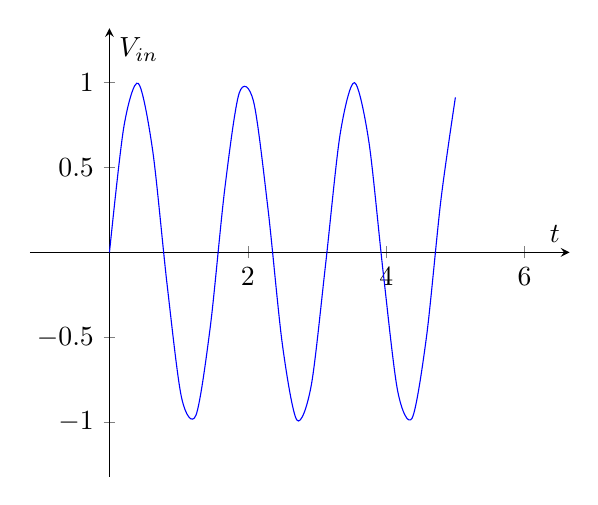
\begin{tikzpicture}
    \begin{axis}[
        domain=0:5,
        axis lines = middle,
        xmin = -0.5,
        xmax = 6,
        ymin = -1.1,
        ymax = 1.1,
        xlabel = $t$,
        ylabel = $V_{in}$,
        enlargelimits = true,
    ]
        \addplot[smooth,mark=none,color=blue] {sin(4*deg(x))};
    \end{axis}
\end{tikzpicture}
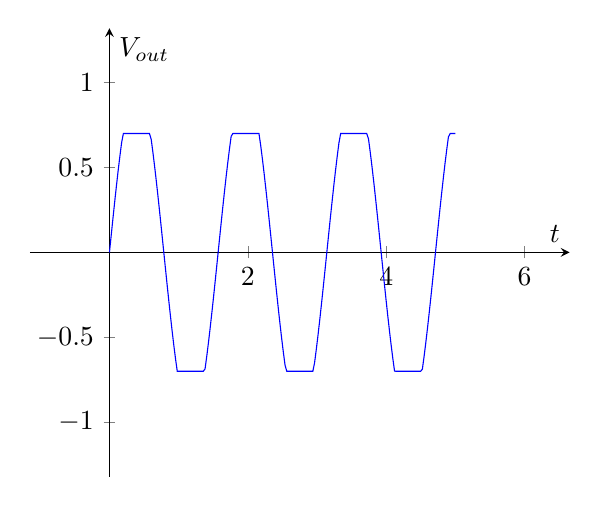
\begin{tikzpicture}
    \begin{axis}[
        domain=0:5,
        axis lines = middle,
        xmin = -0.5,
        xmax = 6,
        ymin = -1.1,
        ymax = 1.1,
        xlabel = $t$,
        ylabel = $V_{out}$,
        enlargelimits = true,
        y filter/.expression={y > 0.7 ? 0.7 : (y < -0.7 ? -0.7 : y)},
    ]
        \addplot[samples=200,mark=none,color=blue] {sin(4*deg(x))};
    \end{axis}
\end{tikzpicture}

  \caption{Impact of the diode limiter on the input sinusoidal voltage. Values that exceed the \SIrange{-0.7}{0.7}{V} range are clamped and the signal is distorted.}
  \label{fig:diode_limiter_signal}
\end{figure}


%%%%%%%%%%%%%%%%%%%%%%%%%%%%%%%%%%%%%%%%%%%%%%%%%%%%%%%%%%%%%%%%%%%%%%%%%%%%%%%%%%%%%%%
\subsection{First-Order Diode Clipper}
%%%%%%%%%%%%%%%%%%%%%%%%%%%%%%%%%%%%%%%%%%%%%%%%%%%%%%%%%%%%%%%%%%%%%%%%%%%%%%%%%%%%%%%
Combining the RC lowpass filter (\Figure{fig:rc_lowpass}) and the diode limiter (\Figure{fig:diode_limiter}) yields the first-order diode clipper (\Figure{fig:diode_clipper_circuit}). It is called "first-order" because only a single capacitor is used \cite{Parker2019}. If the input voltage is within the limiter's operational range, the circuit acts as a lowpass filter. If the voltage exceeds this range, it is clipped at the output and distortion is introduced.

The first-order diode clipper can be described by a nonlinear \ac{ODE} \cite{Yeh2007}
\begin{equation}
  \frac{\mathrm{d} V_\text{out}}{\mathrm{d}t} = \frac{V_\text{in} - V_\text{out}}{RC} - 2 \frac{I_\text{s}}{C} \sinh \left(\frac{V_\text{out}}{V_\text{t}}\right),
  \label{eq:diode_clipper_equation}
\end{equation}
where $V_\text{in}$ is the input voltage, $V_\text{out}$ is the output voltage, $t$ denotes time, $R$ is the serial resistance, $C$ is the parallel capacity, $I_\text{s}$ is the reverse saturation current, and $V_\text{t}$ is the thermal voltage. The last two are parameters of the diodes that can be measured \cite{Yeh2007}.

The parameter values of discrete elements used in the experiments were taken from \cite{Yeh2008}. They are summarized in \Table{tab:diode_clipper_element_parameters}.

\begin{table}
  \centering
  \caption{Parameter values of the discrete elements used in the diode clipper circuit. Source: \cite{Yeh2008}.}
  \begin{tabular}{c|c}
    \toprule
    \textbf{Parameter} & \textbf{Value} \\
    \midrule
    $R$ & \SI{2.2}{k\ohm} \\
    $C$ & \SI{10}{nF} \\
    $I_\text{s}$ & \SI{2.52}{nA} \\
    $V_\text{t}$ & \SI{45.3}{mV} \\
    \hline
  \end{tabular}
  \label{tab:diode_clipper_element_parameters}
\end{table}

$V_\text{in}$ is typically on the order of volts.

%%%%%%%%%%%%%%%%%%%%%%%%%%%%%%%%%%%%%%%%%%%%%%%%%%%%%%%%%%%%%%%%%%%%%%%%%%%%%%%%%%%%%%%
\subsection{Relation to Other Work}
%%%%%%%%%%%%%%%%%%%%%%%%%%%%%%%%%%%%%%%%%%%%%%%%%%%%%%%%%%%%%%%%%%%%%%%%%%%%%%%%%%%%%%%

The first-order diode clipper is a system particularly interesting in the context of ODENet, because it is governed by a known \ac{ODE} \cite{Yeh2007,Yeh2008}. Additionally, it was already modeled using a \ac{ResNet}-like architecture in \cite{Parker2019}. Thus, learning to imitate the diode clipper allowed the validation of ODENet and comparison to 
\begin{itemize}
    \item an \ac{LSTM}-based architecture from \cite{Wrightetal2020},
    \item a \ac{ResNet}-like architecture from \cite{Parker2019}, and
    \item a numerical solution using the \ac{ODE} from \cite{Yeh2007,Yeh2008}.
\end{itemize}

\section{Phaser Modeling}

This section presents the results of phaser modeling in a manner analogous to the diode clipper results presented in the previous section.

%%%%%%%%%%%%%%%%%%%%%%%%%%%%%%%%%%%%%%%%%%%%%%%%%%%%%%%%%%%%%%%%%%%%%%%%%%%%%%%%%%%%%%%
\subsection{Training Data}
\label{sec:phaser_training_data}
%%%%%%%%%%%%%%%%%%%%%%%%%%%%%%%%%%%%%%%%%%%%%%%%%%%%%%%%%%%%%%%%%%%%%%%%%%%%%%%%%%%%%%%

The training data consisted solely of guitar recordings taken from the Fraunhofer IDMT database \cite{Kehling2014}. Some of the recordings were additionally distorted using a software distortion plug-in. The purpose of applying additional distortion was to make the effect of phaser application more audible thanks to the harmonic-rich spectrum of distorted signals. The underlying assumption was that the network would learn better from these more pronounced parts. Additionally, they should make the evaluation task easier during listening tests. 

The acoustic, electric, and distorted guitar recordings were evenly split among the training, validation, and test sets. The training set was 5 minutes 44 seconds long, the validation set was 1 minute 6 seconds long, and the test set was 1 minute 49 seconds long. Audio data was single-channel at \SI{44100}{Hz} sampling rate.

The dataset was synthesized using the digital model of a phaser from \cite{Kiiski2016} with the feedback turned off. The purpose of using synthesized data instead of recorded data was to provide a ground truth LFO signal. This was the approach taken for the initial validation in \cite{Wright2020}. If a recording had been used, we would have needed to estimate the LFO signal, which could obscure the analysis. The LFO signal used for the synthesis was a rectified sine at \SI{17}{Hz}. Again, since the purpose of the training was to validate if the ODENet architecture could be applied to phaser modeling, only one type and rate of the LFO signal were used. If the answer was positive, more LFO waveforms and frequencies would be used (probably involving some not seen during training at test time). 

%%%%%%%%%%%%%%%%%%%%%%%%%%%%%%%%%%%%%%%%%%%%%%%%%%%%%%%%%%%%%%%%%%%%%%%%%%%%%%%%%%%%%%%
\subsection{Training}
\label{sec:phaser_training}
%%%%%%%%%%%%%%%%%%%%%%%%%%%%%%%%%%%%%%%%%%%%%%%%%%%%%%%%%%%%%%%%%%%%%%%%%%%%%%%%%%%%%%%
The training procedure was identical to the one for the diode clipper as described in \Section{sec:diode_clipper_training}. The only difference was that the validation loss was computed every 10 epochs instead of every epoch. 

The loss functions used for the training and the validation were the average distance measures in the time-frequency domain as described in \Section{sec:loss_functions}. Different distance measures allowed to observe different characteristics of ODENet. All models were trained and tested on data at \SI{44100}{Hz} sampling rate.

% It was chosen because of superior validation performance at high frequencies when used to train the baseline (\ac{LSTM}) in comparison to $L_1$ and $L_2$ distances in the \ac{STFT} domain as well as the \ac{ESR}.

%%%%%%%%%%%%%%%%%%%%%%%%%%%%%%%%%%%%%%%%%%%%%%%%%%%%%%%%%%%%%%%%%%%%%%%%%%%%%%%%%%%%%%%
\subsection{Compared Models}
\label{sec:phaser_models}
%%%%%%%%%%%%%%%%%%%%%%%%%%%%%%%%%%%%%%%%%%%%%%%%%%%%%%%%%%%%%%%%%%%%%%%%%%%%%%%%%%%%%%%

In the case of the phaser models, only the ODENet framework was compared to the baseline: an \ac{LSTM} from \cite{Wright2020} with 16 memory cells (\ac{LSTM}16). For the derivative network a sufficiently large \ac{MLP} was chosen. Its dimensionality was $M + 2 \times 30 \times 60 \times 60\times 60 \times 30\times M$, where $M$ was the manually set size of the state vector. The nonlinearity used was \ac{SELU}. To prevent divergence, we added a weight decay term to the loss function as a regularizer.

\begin{table}[]
    \caption{Compared network architectures for phaser modeling}
    \centering
    \begin{tabular}{@{}l|c c @{}}
\toprule
Model & LSTM16 & ODENet \\ \midrule % state_size = 36, hidden_size = 30
Number of   parameters & 1297 & \makecell{11161 (state size 1)\\12198 (state size 18)\\13296 (state size 36)} \\
Weight decay & 1e-7 & 1e-7             \\
Learning rate & 0.001 & 0.0005            \\
Learning rate schedule & none & one cycle LR 0.003      \\
Epochs in training & 1000 & 1200            \\
Hours in training & 3.5 & 22.5           \\
Teacher forcing & never & always       \\ 
Minibatch size & 64 &   256  \\ \bottomrule
\end{tabular}%

    \label{tab:phaser_models_data}
\end{table}

%%%%%%%%%%%%%%%%%%%%%%%%%%%%%%%%%%%%%%%%%%%%%%%%%%%%%%%%%%%%%%%%%%%%%%%%%%%%%%%%%%%%%%%
\subsection{Results and Discussion}
\label{sec:phaser_results}
%%%%%%%%%%%%%%%%%%%%%%%%%%%%%%%%%%%%%%%%%%%%%%%%%%%%%%%%%%%%%%%%%%%%%%%%%%%%%%%%%%%%%%%

The goal of phaser modeling was not only to compare ODENet to the approach taken in \cite{Wright2020} but also to verify the assumption on the state augmentation. The assumption was that the derivative network can use the unobserved entries in the state vector to store information helpful in obtaining more accurate results.

%%%%%%%%%%%%%%%%%%%%%%%%%%%%%%%%%%%%%%%%%%%%%%%%%%%%%%%%%%%%%%%%%%%%%%%%%%%%%%%%%%%%%%%
\subsubsection{The Impact of State Augmentation}
%%%%%%%%%%%%%%%%%%%%%%%%%%%%%%%%%%%%%%%%%%%%%%%%%%%%%%%%%%%%%%%%%%%%%%%%%%%%%%%%%%%%%%%
The effect of augmenting the state vector from 1 to 18 entries when training with the average $L_1$ distance in the \ac{STFT} domain can be seen in \Figure{fig:state_augmentation}. Although no target was provided for the 17 latent entries, the network used them to store meaningful information for each time point. The observed improvement is over two-fold. Therefore, it may be beneficial to augment the state, even if the training signal is not provided for all of its entries. However, the improvement was not observed when $L_2$ or $LSD_\text{RMS}$ distances were used.

\begin{figure}
    \centering
    \begin{tikzpicture}
    \begin{axis}[
        no markers,
        every axis plot/.append style={ultra thick},
        xmin = 0,
        xmax = 1200,
        ymin = 0,
        grid,
        xlabel = Epoch,
        ylabel = Validation Loss,
    ]
        \addplot[smooth,mark=none,color=red] table [x=Step, y=Value, col sep=comma] {figures/tikz/state_augmentation/State_size_1_L1_STFT-tag-Loss_validation.csv};
        \addplot[smooth,mark=none,color=green] table [x=Step, y=Value, col sep=comma] {figures/tikz/state_augmentation/State_size_36_L1_STFT_DerivativeMLP2-tag-Loss_validation.csv};
        \legend{state size 1, state size 18};
    \end{axis}
\end{tikzpicture}

    \caption{Average $L_1$ loss of ODENet in the \ac{STFT} domain on the validation set with and without state augmentation.}
    \label{fig:state_augmentation}
\end{figure}

%%%%%%%%%%%%%%%%%%%%%%%%%%%%%%%%%%%%%%%%%%%%%%%%%%%%%%%%%%%%%%%%%%%%%%%%%%%%%%%%%%%%%%%
\subsubsection{Comparison to the Baseline}
%%%%%%%%%%%%%%%%%%%%%%%%%%%%%%%%%%%%%%%%%%%%%%%%%%%%%%%%%%%%%%%%%%%%%%%%%%%%%%%%%%%%%%%

Test results of phaser modeling are shown in \Table{tab:phaser_results}, where $LSD_\text{RMS}$ was defined in \Equation{eq:log_spectral_distance}, \ac{segSNR} was defined in \Equation{eq:seg_snr}, and \ac{PEAQ} was explained in \Section{subsec:va_evaluation}. The $LSD_\text{RMS}$  loss was chosen for the final training and comparison, because during a visual inspection of the magnitude \ac{STFT} it resulted in the best match of phaser notches in the output signal of the baseline model. It was assumed that it would enable effective learning for ODENet as well.

\begin{table}[]
    \caption{Test results of the phaser models.}
    \centering
    \newcommand{\modelNameCellWidth}{1.8cm}
    \begin{tabular}{@{} l | c c @{}}
        \toprule
        Model & LSTM16 & ODENet \\ \midrule
        Loss    & \textbf{4.7\%} & TBF \\
        segSNR  & \textbf{8.5} & TBF  \\
        ODG     & \textbf{-0.27} & TBF \\ \bottomrule
    \end{tabular}%
    
    \label{tab:phaser_results}
\end{table}

In terms of numerical measures, \ac{LSTM}16 significantly outperformed ODENet. The validation curves of both models can be seen in \Figure{fig:phaser_lstm_vs_fe}. \ac{LSTM}16 has smaller dynamics of learning, which could point to the fact that it is more suited for modeling the phaser.

\begin{figure}
    \centering
    \begin{tikzpicture}
    \begin{axis}[
        no markers,
        every axis plot/.append style={ultra thick},
        xmin = 0,
        xmax = 1200,
        ymin = 0,
        grid,
        xlabel = Epoch,
        ylabel = Validation Loss,
    ]
        \addplot[smooth,mark=none,color=blue] table [x=Step, y=Value, col sep=comma] {figures/tikz/phaser_lstm_vs_fe/LSTM_L1_STFT.csv};
        \addplot[smooth,mark=none,color=green] table [x=Step, y=Value, col sep=comma] {figures/tikz/phaser_lstm_vs_fe/FE_L1_STFT.csv};
        \legend{LSTM16, ODENet};
    \end{axis}
\end{tikzpicture}

    \caption{Average $LSD_\text{RMS}$ of the compared models on the validation set.}
    \label{fig:phaser_lstm_vs_fe}
\end{figure}

The results in the \ac{STFT} domain can be seen in \Figure{fig:phaser_test_spectrograms}. The notches learned by \ac{LSTM}16 closely match those of the target. The notches learned by ODENet are almost invisible (although they are present at closer inspection). It must also be stated that ODENet always diverged during test, what can be seen in the range of values in the colorbar.

\newcommand{\scaleboxsizee}{0.8}
\begin{figure}
    \centering
    \begin{subfigure}{0.7\textwidth}
        \centering
        \scalebox{0.81}{% This file was created by tikzplotlib v0.9.6.
\begin{tikzpicture}

\begin{axis}[
colorbar,
colorbar style={ytick={-40,-20,-7.105427357601e-15,20},yticklabels={\(\displaystyle -40\),\(\displaystyle -20\),\(\displaystyle 0\),\(\displaystyle 20\)},ylabel={}},
colormap/viridis,
point meta max=22.9006375273498,
point meta min=-54.103633370184,
tick align=outside,
tick pos=left,
x grid style={white!69.0196078431373!black},
xlabel={Time [s]},
xmin=0, xmax=14.9072108843537,
xtick style={color=black},
xtick={0,5,10,15},
xticklabels={\(\displaystyle 0\),\(\displaystyle 5\),\(\displaystyle 10\),\(\displaystyle 15\)},
y grid style={white!69.0196078431373!black},
ylabel={Frequency [kHz]},
ymin=0, ymax=22,
ytick style={color=black},
ytick={0,5,10,15,20,25},
yticklabels={\(\displaystyle 0\),\(\displaystyle 5\),\(\displaystyle 10\),\(\displaystyle 15\),\(\displaystyle 20\),\(\displaystyle 25\)}
]
\addplot graphics [includegraphics cmd=\pgfimage,xmin=0, xmax=14.9072108843537, ymin=0, ymax=22] {figures/tikz/phaser_test_spectrograms/FameSweetToneOffNoFb-test-target_stft-000.png};
\end{axis}

\end{tikzpicture}
}
    \end{subfigure}
    \begin{subfigure}{0.7\textwidth}
        \centering
        \scalebox{\scaleboxsizee}{% This file was created by tikzplotlib v0.9.6.
\begin{tikzpicture}

\begin{axis}[
colorbar,
colorbar style={ytick={-40,-20,0,20},yticklabels={\(\displaystyle -40\),\(\displaystyle -20\),\(\displaystyle 0\),\(\displaystyle 20\)},ylabel={Magnitude [dB]}},
colormap/viridis,
point meta max=21.1321993583666,
point meta min=-55.5277115981883,
tick align=outside,
tick pos=left,
x grid style={white!69.0196078431373!black},
xlabel={Time [s]},
xmin=0, xmax=14.9072108843537,
xtick style={color=black},
xtick={0,5,10,15},
xticklabels={\(\displaystyle 0\),\(\displaystyle 5\),\(\displaystyle 10\),\(\displaystyle 15\)},
y grid style={white!69.0196078431373!black},
ylabel={Frequency [kHz]},
ymin=0, ymax=22,
ytick style={color=black},
ytick={0,5,10,15,20,25},
yticklabels={\(\displaystyle 0\),\(\displaystyle 5\),\(\displaystyle 10\),\(\displaystyle 15\),\(\displaystyle 20\),\(\displaystyle 25\)}
]
\addplot graphics [includegraphics cmd=\pgfimage,xmin=0, xmax=14.9072108843537, ymin=0, ymax=22] {figures/tikz/phaser_test_spectrograms/LSTM16_log_spectral_distance_stft-000.png};
\end{axis}

\end{tikzpicture}
}
    \end{subfigure}
    \begin{subfigure}{0.7\textwidth}
        \centering
        \scalebox{\scaleboxsizee}{% This file was created by tikzplotlib v0.9.6.
\begin{tikzpicture}

\begin{axis}[
colorbar,
colorbar style={ytick={-60,-40,-20,0,20,40},yticklabels={\(\displaystyle -60\),\(\displaystyle -40\),\(\displaystyle -20\),\(\displaystyle 0\),\(\displaystyle 20\),\(\displaystyle 40\)},ylabel={Magnitude [dB]}},
colormap/viridis,
point meta max=49.2661401752569,
point meta min=-61.6565473918622,
tick align=outside,
tick pos=left,
x grid style={white!69.0196078431373!black},
xlabel={Time [s]},
xmin=0, xmax=14.9072108843537,
xtick style={color=black},
xtick={0,5,10,15},
xticklabels={\(\displaystyle 0\),\(\displaystyle 5\),\(\displaystyle 10\),\(\displaystyle 15\)},
y grid style={white!69.0196078431373!black},
ylabel={Frequency [kHz]},
ymin=0, ymax=22,
ytick style={color=black},
ytick={0,5,10,15,20,25},
yticklabels={\(\displaystyle 0\),\(\displaystyle 5\),\(\displaystyle 10\),\(\displaystyle 15\),\(\displaystyle 20\),\(\displaystyle 25\)}
]
\addplot graphics [includegraphics cmd=\pgfimage,xmin=0, xmax=14.9072108843537, ymin=0, ymax=22] {figures/tikz/phaser_test_spectrograms/FE_log_spectral_distance_stft-001.png};
\end{axis}

\end{tikzpicture}
}
    \end{subfigure}
    \caption{A fragment of the magnitude \ac{STFT} of the models' test output. (Top) Target. (Middle) \ac{LSTM}16. (Bottom) ODENet (state size 36).}
    \label{fig:phaser_test_spectrograms}
\end{figure}

In casual listening, \ac{LSTM}16 sounds indistinguishable from the target. On the contrary, the output of ODENet does not sound as processed with phaser at all. The gentle notches that can be seen under a close inspection of ODENet output spectrograms are not audible.

Ultimately, we were not able to achieve a better performance of ODENet on the phaser dataset. This suggests that ODENet may not be able to learn the instantaneous derivative of the phaser system.

%%%%%%%%%%%%%%%%%%%%%%%%%%%%%%%%%%%%%%%%%%%%%%%%%%%%%%%%%%%%%%%%%%%%%%%%%%%%%%%%%%%%%%%
\section{Evaluation Metrics}
\label{subsec:va_evaluation}
%%%%%%%%%%%%%%%%%%%%%%%%%%%%%%%%%%%%%%%%%%%%%%%%%%%%%%%%%%%%%%%%%%%%%%%%%%%%%%%%%%%%%%%

An important part of \ac{VA} modeling is the assessment of how well the model imitates the original device. The quality of the \ac{VA} algorithm can be assessed objectively (using a similarity or distance measure between the outputs of the model and the device for a given input signal) or subjectively (using a listening test involving human participants). 

In this work, a few objective measures between the target signal (device output) and the model were used. The subjective evaluation has been left for future work. One of the employed measures was the \ac{ESR} described in \Section{sec:loss_functions}.
The \ac{ESR} is a distance measure that is minimized during neural network training and used as a validation and test metric. We may, however, employ a different objective measure at test time than at training time. The reasons for this are that not all measures are suited to neural network training and that different objective measures let us assess different aspects of the model.

For the assessment of the models in this work, especially their aliasing behavior, an objective measure from the domain of speech enhancement was used. The \ac{segSNR} is an average signal-to-noise ratio across segments of the system-undery-study output $s[n]$ and the model output $\hat{s}[n]$ \cite{Hansen98}

\begin{equation}
    \text{segSNR}(s, \hat{s}) = \frac{1}{M} \sum \limits_{m=0}^{M-1} 10 \log_{10} \left( \frac{\sum_{n=0}^{N-1} (s[n+mR])^2}{\sum_{n=0}^{N-1} (\hat{s}[n+mR] - s[n+mR])^2} \right),
    \label{eq:seg_snr}
\end{equation}

where $m$ is the frame index, $R$ is the number of samples between successive frames, $N$ is the frame length, and $M$ is the number of frames.

% The \ac{fw-segSNR} is a perceptually motivated objective measure that uses a weighted average and a time-frequency representation \cite{Hu2008}

% \begin{equation}
%     \text{fw-segSNR}(s, \hat{s}) = \frac{10}{M} \sum \limits_{m=0}^{M-1} \frac{ \sum_{j=1}^{K} W(j,m) \log_{10} \left( \frac{|S(j,m)|^2}{(|S(j,m)|-|\hat{S}(j,m)|)^2} \right)}{\sum_{j=1}^{K} W(j,m)},
% \end{equation}
% where $W(j,m)$ is the weight assigned to the $j$-th frequency band, $K$ is the number of bands, $m$ is the frame index, $M$ is the number of frames, $|S(j,m)|$ is the magnitude of a Gaussian window-weighted target signal spectrum in the $j$-th frequency band and at the $m$-th frame, and $|\hat{S}(j,m)|$ is the same value computed for the signal from the model. Additionally,

% \begin{equation}
%     W(j,m) = |S(j,m)|^{0.2}.
% \end{equation}

% The frequency bands are spaced according to the 25 critical bands of the ear spanning the range \SIrange{50}{3597.63}{Hz}. Therefore, only frequencies up to \SI{4000}{Hz} are taken into consideration although the frequencies above are still relevant for musical perception.

For computing \ac{segSNR} we used a Python implementation available on GitHub\footnote{\url{https://github.com/schmiph2/pysepm}, retrieved 05.08.2021.}.

\Ac{segSNR} is different from \ac{ESR} in that it measures the relative similarity between the target and the model signals (the higher the obtained value the more accurate the model) and that it works in a frame-wise fashion. \ac{segSNR} allows large local errors to influence the overall measure more than the \ac{ESR}, which has high correlation with the subjective quality when it comes to speech signals \cite{Hansen98}. That is why it was chosen for this work: as a temporary substitute for the listening tests.

The other objective measure used was the \ac{ODG} from the \ac{ITU} recommendation \cite{ITU1387}. 
Results obtained from \ac{ODG} are often referred to as \acs{PEAQ} which stands for "\acl{PEAQ}". However, the acronym is often translated into "Perceptual Evaluation of Audio Quality", a name not present in the recommendation. The goal of \acs{PEAQ} is to approximate the results of a subjective evaluation via listening tests. In the listening tests, the subjects evaluate the impairment of the presented signals with respect to a known reference signal. The given score is termed \ac{SDG}. Both, \ac{ODG} and \ac{SDG}, are continuous-valued numbers from -4 to 0, where 0 means that the degradation from the reference is imperceptible and -4 means that the impairment is very annoying. These grades are ultimately converted to the ITU-R five-grade impairment scale \cite{ITU1387}. All of them are presented in \Table{tab:itu_impairment_scale}.

\begin{table}
  \centering
  \begin{tabular}{c c}
    \toprule
    \textbf{Grade} & \textbf{Degradation description} \\ \midrule
    5.0 & Imperceptible \\
    4.0 & Perceptible but not annoying \\
    3.0 & Slightly annoying \\
    2.0 & Annoying \\
    1.0 & Very annoying\\ \bottomrule
  \end{tabular}
  \caption{The ITU-R five-grade impairment scale.}
  \label{tab:itu_impairment_scale}
\end{table}

As the procedure for calculating \ac{ODG} is quite complex, we used a ready-made implementation by Giuseppe Gottardi\footnote{\url{https://github.com/akinori-ito/peaqb-fast}, retrieved 07.08.2021.}. As \acs{PEAQ} cannot replace actual listening tests, it is used in this work as an unbinding reference metric.


